% Section content template for individual Educative lessons
% This file contains the actual content for a specific section
% Generated from Educative API section content

% Section: Getting Ready: The Meeting Scheduler Problem
% Section ID: 5571997574889472
% Section Slug: getting-ready-the-meeting-scheduler-problem
% Generated: 2025-12-12T13:05:42.094846

\subsection{Problem definition}\label{wqzw3-1bB9gP-uGZtnIp8-1}
\\
A \textbf{meeting scheduler} software enables organizations to efficiently arrange and manage meetings for multiple participants, ensuring optimal use of meeting rooms and everyone's time. The system helps find a suitable time and location by checking participants' availability, room capacity, and preferences. Organizers and participants can book, update, or cancel meetings; add or remove attendees; and receive real-time notifications for all meeting changes. When participants respond to invites or remove themselves from a meeting, their calendars are automatically updated to reflect their participation status.
\\
In this LLD interview case study, you'll focus on:

\begin{itemize}
\item
\protect\phantomsection\label{_OKyNwb9JcVkc1l_oSAJ4}
Assigning available meeting rooms based on room capacity, schedule, and participant count.
\item
\protect\phantomsection\label{FHReYFuSrnvsgLVQ6cg6L}
Determining optimal meeting times by analyzing the availability of all required attendees.
\item
\protect\phantomsection\label{Mq8tNC_NTC29sZjjgdqca}
Managing the full meeting life cycle: creation, updates, cancellations, and participant management.
\item
\protect\phantomsection\label{4cwBqt3PRrbfOFwXEpiop}
Sending notifications for all meeting-related events, and updating calendars automatically when meetings are accepted, declined, or modified.
\item
\protect\phantomsection\label{XXlMC7zehaI63fsROdUTB}
Tracking each participant's invite/response status in the meeting record, and handling changes such as removals, cancellations, and overlapping bookings.
\end{itemize}
\\
\textbf{Note:} This system model applies to any organization or platform that requires collaborative meeting management, from startups to enterprise-level operations.

\begin{figure}[htbp]
 \centering
 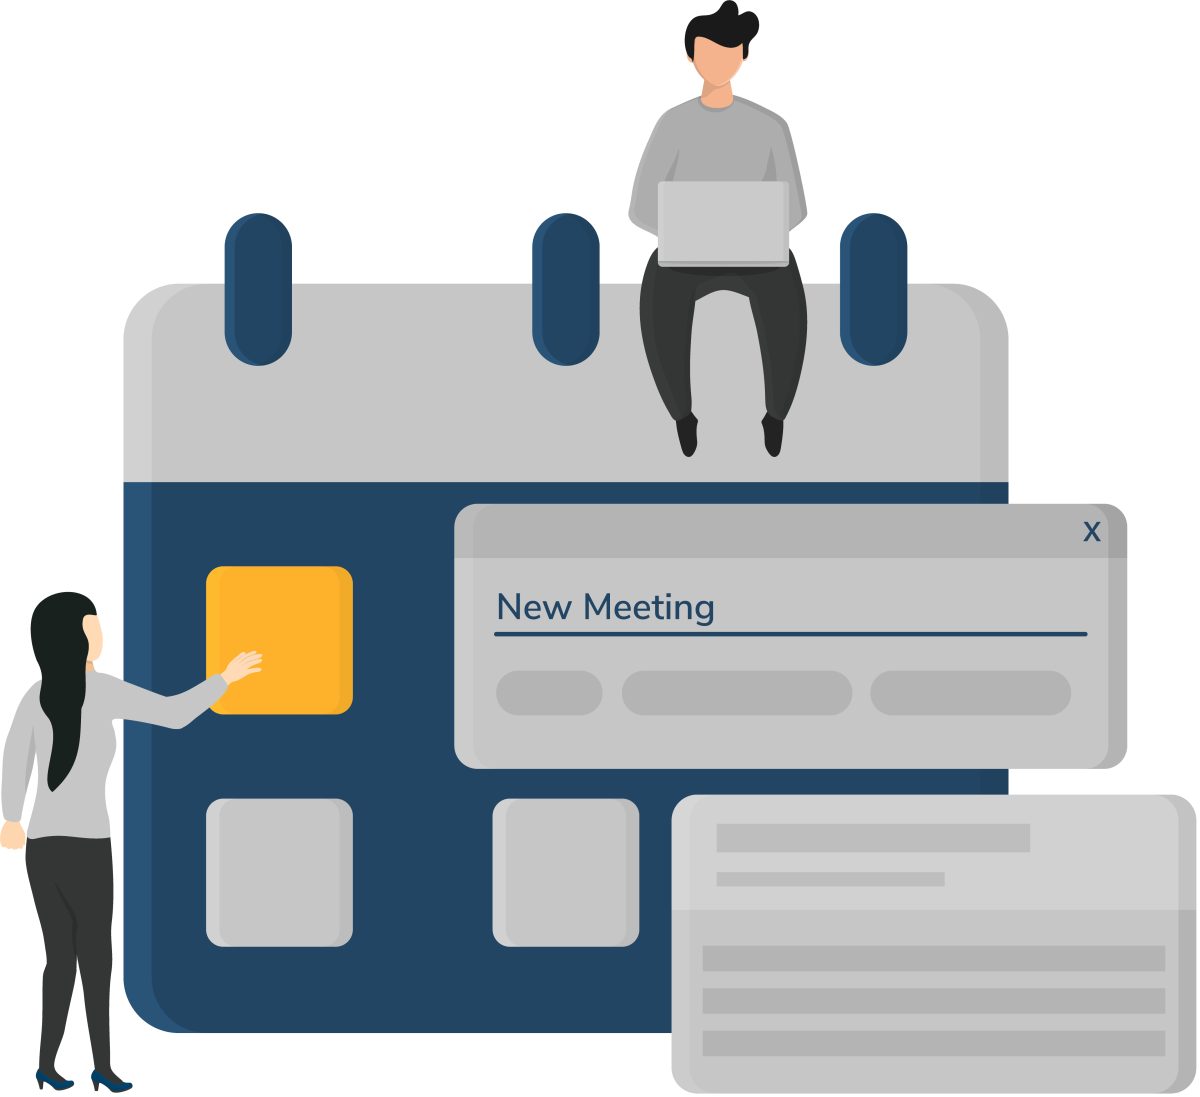
\includegraphics[width=0.15\textwidth]{Images/chapter_13/section_5571997574889472/6411209551380480.png}
 \caption{Schedule a meeting using a meeting scheduler}
\end{figure}

\subsection{Expectations from the interviewee}\label{wqzw3-1bB9gP-uGZtnIp8-2}
\\
It is important to narrow down the components you will include in your design of a meeting scheduler. The following section provides an overview of some of the main expectations the interviewer will want to hear you discuss in more detail during the interview.

\subsubsection{Room assignment}\label{Aps3b3Rs9CFNU3XZXnKoG}
\\
A meeting scheduler assigns a meeting room to a scheduled meeting. Make sure to ask the following questions of the interviewer to figure out how this assignment works:

\begin{itemize}
\item
\protect\phantomsection\label{-PLIkZT7gYBw8s99CPYuN}
How does the system determine available rooms?
\item
\protect\phantomsection\label{f0cbhYRmI-GfZo5F2m4i6}
How important is the capacity of a room when assigning a room for a meeting?
\end{itemize}

\subsubsection{Availability of attendees}\label{3PhtpjsDC3HeZ2V99Gl38}
\\
Multiple attendees are in a meeting, and all attendees have different schedules. You may ask the following questions to understand how the scheduler works:

\begin{itemize}
\item
\protect\phantomsection\label{Dw-w4v-bRN6dsW7umX49d}
How does the system check the availability of the attendees?
\item
\protect\phantomsection\label{giIyR4boRtJ_es-qSs5lt}
How does the system access the meeting information of all attendees?
\end{itemize}

\subsection{Design approach}\label{FgxX72eGTi7TExvcDCSho}
\\
We will design this meeting scheduler system using the bottom-up design approach. For this purpose, we will follow the steps below:

\begin{itemize}
\item
\protect\phantomsection\label{cHCIsn1GX6asIsQACRHgb}
First, we'll identify the simple core entities such as \texttt{MeetingRoom}, \texttt{Interval}, \texttt{Participant}, and \texttt{Calendar}, and define their responsibilities and relationships.
\item
\protect\phantomsection\label{a70YXyWljHI9SsVwrCNzB}
Next, we'll model how meetings are created, how the scheduler checks room and participant availability, assigns suitable rooms, and sends notifications for bookings, cancellations, and updates.
\item
\protect\phantomsection\label{oFkliksAkD8GFicdDBSPs}
We'll ensure the design gracefully handles conflicts, last-minute updates, recurring meetings, and edge cases like overlapping events or room shortages.
\item
\protect\phantomsection\label{5eQRjIuu0f75ulHXRgTZN}
This approach will incorporate SOLID principles and design patterns, ensuring the system is scalable, maintainable, and adaptable to future needs.
\end{itemize}
\\
Diagrams and sample code will illustrate the main workflows, class structures, and collaboration between entities.

\subsection{Design pattern~}\label{EFFv6G5Afm3ipxuO7os5A}
\\
During an interview, discussing the design patterns the meeting scheduler falls under is always a good practice. Stating the design patterns gives the interviewer a positive impression and shows that the interviewee is well-versed in the advanced concepts of object-oriented design.
\\
Try to answer the following question. If you are not familiar with design patterns, don't worry! You can learn about them by asking, ``Define design patterns.''

\textbf{Question:}

Which design pattern(s) should be used to design a meeting scheduler? Please elaborate on your choice(s).

Let's explore the requirements of the meeting scheduler in the next lesson.

% End of section content